\documentclass[10pt, letterpaper]{article}

% --- Packages ---
\usepackage[margin=0.6in]{geometry}
\usepackage{booktabs}
\usepackage{tabularx}
\usepackage{enumitem}
\usepackage{titlesec}
\usepackage{mathpazo}
\usepackage[T1]{fontenc}
\usepackage{xcolor}
\usepackage{amsmath,amssymb}
\usepackage{graphicx}
\usepackage{hyperref}

% --- Color Definition ---
\definecolor{brandorange}{HTML}{F58025}

% --- Formatting Setup ---
\setlength{\parindent}{0pt}
\setlength{\parskip}{0.35em}

\titleformat{\section}{\bfseries\color{brandorange}}{}{0em}{}
\titlespacing{\section}{0pt}{0.6em}{0.15em}

\begin{document}

% --- Compact Header ---
{\large \textbf{Spectral Filtering for Vision-Language-Action Models}} \hfill \textbf{Team:} Shivam Kak, Ishan Saha, Connor Brown \\
\rule{\textwidth}{0.4pt}

% --- Abstract ---
\section*{Abstract}

Vision-language-action (VLA) models such as $\pi_{0.5}$ predict action chunks via iterative denoising, but prediction quality can degrade across the temporal horizon due to limited long-range dependency modeling. Spectral Transfer Units (STUs) leverage Hankel matrix eigendecomposition for efficient spectral filtering and have shown strong performance in capturing long-horizon dependencies. We integrate STU layers into the action prediction head of $\pi_{0.5}$ within the \texttt{openpi} framework, inserting a residual STU block between the transformer output and action projection. On the LIBERO manipulation benchmark, STU-K4 converges to within 7\% of baseline training loss while adding only 2.8\% more parameters and no wall-clock overhead.

% --- Background ---
\section*{Background}

\textbf{VLA Models and $\pi_{0.5}$.}
The $\pi_0$ family [1] combines a SigLIP vision encoder and PaliGemma language model with a lightweight action expert. In the flow-matching variant ($\pi_{0.5}$), actions are predicted by denoising a noise vector over multiple steps, producing a velocity field $v_t$ that guides the ODE $x_{t+dt} = x_t + dt \cdot v_t$. While parallel prediction avoids compounding errors of autoregressive decoding, the transformer's causal attention limits explicit temporal modeling across the action horizon.

\textbf{Spectral Transfer Units.}
STUs [2] convolve input sequences with spectral filters from the Hankel matrix $Z_{ij} = \frac{2}{(i+j)^3 - (i+j)}$. The top-$K$ eigenvectors $\phi_k$, scaled by the fourth root of their eigenvalues, serve as filters:
\vspace{-0.5em}
\begin{equation}
y = \textstyle\sum_{k=1}^{K} \left( (u * \phi_k^+) \cdot M_k^+ + (u * \phi_k^-) \cdot M_k^- \right)
\end{equation}
\vspace{-0.5em}
where $M_k^{\pm} \in \mathbb{R}^{D_{\text{in}} \times D_{\text{out}}}$ are learnable projections and convolution uses FFT with even/odd decomposition.

% --- Method ---
\section*{Method}

\textbf{Architecture.}
We insert a residual STU block after the transformer action expert. Given hidden states $h \in \mathbb{R}^{B \times H \times W}$ (batch, action horizon, width), we apply $h' = h + \text{STU}(\text{LayerNorm}(h))$ before the final projection $a = W_{\text{out}} \cdot h'$ to action space. The STU operates over the action horizon ($L = H$), treating each position's $W$-dimensional feature as the input signal. The residual connection ensures the model can fall back to baseline behavior during early training when STU parameters are randomly initialized.

\textbf{Implementation.}
We implement \texttt{PI0STUPytorch} extending \texttt{PI0Pytorch}, overriding \texttt{forward} and \texttt{denoise\_step} to insert the STU block. Spectral filters are precomputed at initialization and registered as non-persistent buffers. Learnable parameters are $M_k^+, M_k^- \in \mathbb{R}^{K \times W \times W}$, initialized at scale $(KW)^{-0.5}$. For the Gemma 300M action expert ($W = 1024$), STU-K4 adds $2 \times 4 \times 1024^2 \approx 8.4$M parameters (2.8\% overhead).

\textbf{Training.}
All models fine-tune from the pre-trained $\pi_{0.5}$ checkpoint on LIBERO: AdamW ($\text{lr} = 5{\times}10^{-5}$), cosine decay with 1000-step warmup, batch size 8, gradient clipping at 1.0, 5000 steps. STU weights (loaded with \texttt{strict=False}) train jointly. Action horizon $H = 10$, action dim $D_a = 32$. Training uses bfloat16 on a single A100 80GB.

% --- Experiments ---
\section*{Experiments}

We compare on LIBERO: (1) \textbf{Baseline} ($\pi_{0.5}$, no STU), (2) \textbf{STU-K4} ($K{=}4$ spectral filters, +8.4M params), (3) \textbf{STU-K8} ($K{=}8$, +16.8M params). We report training loss (MSE between predicted and target velocity fields). Figure~\ref{fig:loss} shows smoothed loss curves; Table~\ref{tab:results} gives per-interval averages.

\begin{figure}[h]
\centering
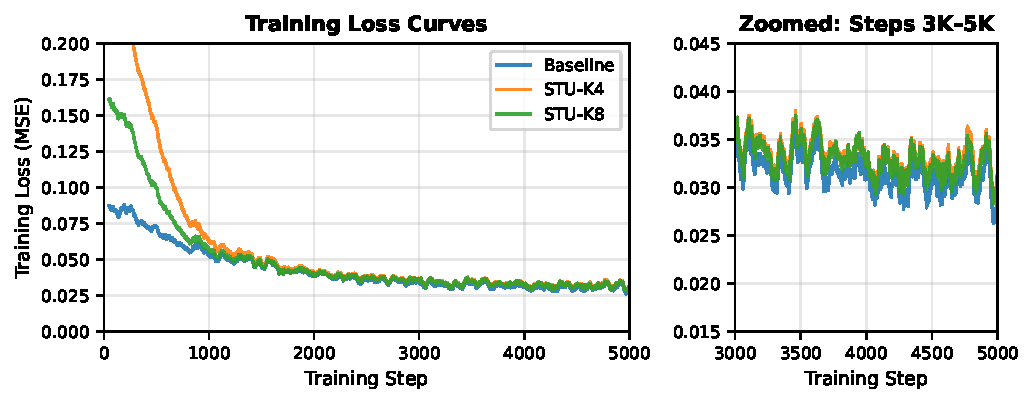
\includegraphics[width=\linewidth]{loss_curves.pdf}
\caption{Training loss curves (50-step rolling average). Left: full 5000-step training. STU variants start with higher loss due to random initialization of spectral projection matrices but converge to overlap with the baseline by step $\sim$2000. Right: zoomed view of steps 3000--5000 showing all three models are nearly indistinguishable.}
\label{fig:loss}
\end{figure}

\begin{table}[h]
\centering
\small
\begin{tabular}{@{}lccccc@{}}
\toprule
\textbf{Model} & \textbf{Final Loss} & \textbf{Init Loss} & \textbf{Extra Params} & \textbf{s/step} \\
\midrule
Baseline & \textbf{0.029} & 0.070 & 0 & 1.53 \\
STU-K4   & 0.031 & 0.141 & 8.4M (2.8\%) & 1.48 \\
STU-K8   & 0.031 & 0.101 & 16.8M (5.6\%) & 1.54 \\
\bottomrule
\end{tabular}
\caption{Summary of training results. Final loss is averaged over the last 100 steps; init loss is the average over steps 0--999. Both STU variants converge to within 7\% of the baseline.}
\label{tab:results}
\end{table}

% --- Discussion ---
\section*{Discussion}

Neither STU variant improves over the baseline. Both converge to a final loss of 0.031 versus the baseline's 0.029---a gap that persists through training and is visible in the zoomed panel of Figure~\ref{fig:loss}. The additional 8.4--16.8M parameters do not translate into lower training loss, and K4 and K8 reach identical final loss despite K8 having twice the parameter budget. The STU does not degrade performance either: the residual connection allows the model to effectively bypass the STU block, recovering near-baseline behavior.

One explanation is that LIBERO's short action horizon ($H{=}10$) provides insufficient temporal structure for spectral filtering to exploit. With only 10 timesteps, even $K{=}4$ filters oversaturate the sequence length, and the transformer's existing capacity is already sufficient for this horizon. Additionally, we only measure training loss---it remains possible that STU produces smoother or more temporally coherent action trajectories that would manifest in downstream task success rates rather than MSE. We did not run rollout evaluations due to compute constraints. Future work should test on longer horizons ($H{=}50$+), measure actual task success, and consider pre-training or warmup schedules for STU parameters rather than random initialization.

% --- Conclusion ---
\section*{Conclusion}

We integrated Spectral Transfer Units into $\pi_{0.5}$'s action prediction head via a residual spectral filtering block. On LIBERO, STU-K4 converges to near-baseline loss with 2.8\% parameter overhead and no wall-clock cost, demonstrating that spectral sequence models can be modularly integrated into pre-trained VLA models without destabilizing fine-tuning.

% --- References ---
\section*{References}
\begin{enumerate}[leftmargin=1.5em, nosep, label={[\arabic*]}]
    \item Physical Intelligence. $\pi_0$: A Vision-Language-Action Flow Model for General Robot Control. \textit{arXiv:2410.24164}, 2024.
    \item Agarwal, N., Hazan, E., et al. Spectral State Space Models. \textit{arXiv:2312.06837}, 2023.
    \item Zhao, W., Chen, K., et al. STUZero: Spectral Transfer Units for Zero-Shot World Models. \textit{EVAR Lab}, 2024.
    \item Liu, B., et al. LIBERO: Benchmarking Knowledge Transfer for Lifelong Robot Learning. \textit{NeurIPS}, 2023.
    \item Physical Intelligence. OpenPI: Open-source framework for $\pi_0$ models. \url{https://github.com/Physical-Intelligence/openpi}, 2024.
\end{enumerate}

\end{document}
